\documentclass{beamer}

\mode<presentation> {

\usetheme{Madrid}


\usecolortheme{whale}


%\setbeamertemplate{footline} % To remove the footer line in all slides uncomment this line
%\setbeamertemplate{footline}[page number] % To replace the footer line in all slides with a simple slide count uncomment this line

%\setbeamertemplate{navigation symbols}{} % To remove the navigation symbols from the bottom of all slides uncomment this line

}

\usepackage{subfig}

%encoding
%--------------------------------------
\usepackage[utf8]{inputenc}
\usepackage[T1]{fontenc}
%--------------------------------------
 
%Portuguese-specific commands
%--------------------------------------
\usepackage[portuguese]{babel}
%--------------------------------------
 
%Hyphenation rules
%--------------------------------------
\usepackage{hyphenat}
\hyphenation{mate-mática recu-perar}
%--------------------------------------

\usepackage{minted}


\usepackage{graphicx} % Allows including images

\graphicspath{{images/}}

\usepackage{booktabs} % Allows the use of \toprule, \midrule and \bottomrule in tables


\usepackage{hyperref}

\usepackage{epigraph}
\usepackage{ragged2e}

\usepackage{bussproofs}
\usepackage{bpextra}
 
\urlstyle{same}

%----------------------------------------------------------------------------------------
%	TITLE PAGE
%----------------------------------------------------------------------------------------

\title[Propositions as Types]{Proposições como Tipos} % The short title appears at the bottom of every slide, the full title is only on the title page

\author{Marcos Benevides} % Your name
\institute[UFMA] % Your institution as it will appear on the bottom of every slide, may be shorthand to save space
{
Universidade Federal do Maranhão \\ % Your institution for the title page
\medskip
\textit{marcos.schonfinkel@gmail.com}\\ % Your email address

\vspace*{2\baselineskip}
GELF - Grupo de Estudos em Lógica e Filosofia Formal

\vspace*{6\baselineskip}

Baseado no artigo original \cite{wadlertypes15} e apresentação de Philip Wadler.
}
\date{\today} % Date, can be changed to a custom date

\begin{document}

\begin{frame}
\titlepage % Print the title page as the first slide
\end{frame}


\begin{frame}[t, allowframebreaks]
\frametitle{Overview}
\tableofcontents
\end{frame}

%----------------------------------------------------------------------------------------
%	PRESENTATION SLIDES
%----------------------------------------------------------------------------------------

%------------------------------------------------
\section{Introdução}
%------------------------------------------------

\begin{frame}{}

\begin{exampleblock}{}
\justifying
  {\large ``Propositions as Types is a notion with depth. It describes a correspondence between a given logic and a given programming language.''}
  \vskip5mm
  \hspace*\fill{\small--- Propositions as Types, Wadler}
\end{exampleblock}

\end{frame}



%------------------------------------------------


\subsection{A Placa Pioneer}

\begin{frame}{A Placa Pioneer}

\begin{figure}
 \centering
 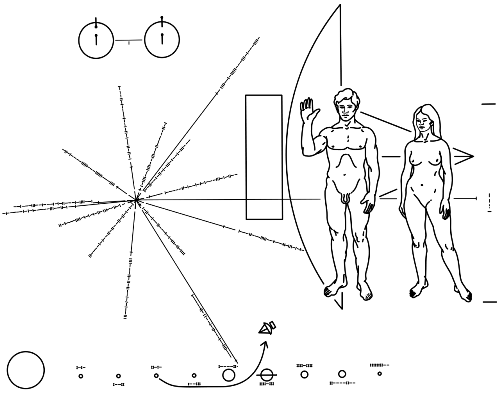
\includegraphics[width=0.8\textwidth]{Pioneer_plaque.png}
\end{figure}

\end{frame}

%------------------------------------------------

\subsection{Algoritmos}

\begin{frame}{Algoritmos}

\begin{figure}
    \centering
    \subfloat[Euclides (325–265 BCE)]{{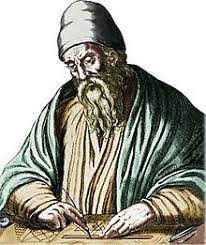
\includegraphics[width=5cm]{euclid.jpeg} }}%
    \qquad
    \subfloat[Al-Khwarizmi (780–850 CE)]{{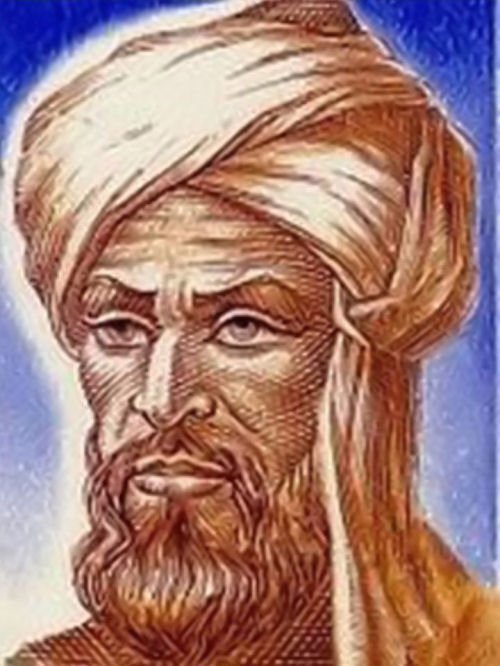
\includegraphics[width=5cm]{al-khwarizmi.png} }}%
\end{figure}

\end{frame}

%------------------------------------------------

\subsection{Computabilidade}

\begin{frame}{Computabilidade}

\begin{block}{}

Apesar de ser uma idéia antiga, definições formais só foram aparecer a partir do Séc. XX.

\begin{itemize}
\item Alonzo Church: $\lambda$-Cálculo (1935)

\cite{church1936unsolvable}

\item Kurt Gödel: Funções Recursivas (1935)

Propostas por Gödel em Princeton e publicadas por Kleene em \cite{kleene1936general}

\item Alan Turing: Máquinas de Turing  (1936)

\cite{turing1937computable}

\end{itemize}

\end{block}

\end{frame}

%------------------------------------------------

\subsection{O programa de Hilbert}

\begin{frame}{Por que isso aconteceu?}

\begin{figure}
    \centering
    \subfloat[David Hilbert]{{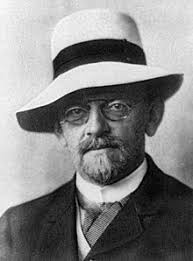
\includegraphics[width=4cm]{hilbert.jpeg} }}%
    \qquad
    \subfloat[Entscheidungsproblem]{{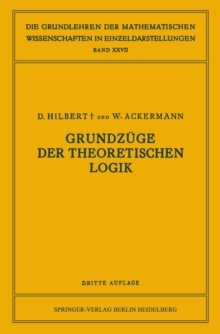
\includegraphics[width=4cm]{eproblem.jpg} }}%
\end{figure}

\end{frame}

%------------------------------------------------

\begin{frame}{Por que isso aconteceu?}
\justifying
Um dos objetivos do Programa de Hilbert era resolver o Entscheidungsproblem (problema de decisão), ou seja, desenvolver um procedimento "efetivamente calculável" para determinar a verdade ou a falsidade de qualquer proposição.\linebreak

\pause

Mas para resolver o Entscheidungsproblem é necessário uma definição formal de "efetivamente cálculável".

\end{frame}

%------------------------------------------------
\section{Dedução Natural}
%------------------------------------------------

\begin{frame}{Dedução Natural}
\begin{columns}
\column{0.38\linewidth}
\centering
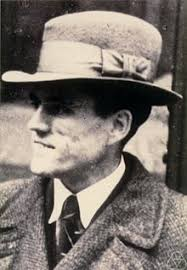
\includegraphics[width=4cm]{gentzen.jpeg}
\column{0.58\linewidth}
\textbf{Gerhard Gentzen, 1909 - 1945.}\\
\justifying
First I wanted to construct a formalism which comes as close as possible to actual reasoning.  Thus arose a “calculus of natural deduction”.
\end{columns} 
\end{frame}

%------------------------------------------------

\begin{frame}{Dedução Natural}

\begin{block}{Introdução}

A notação

\begin{prooftree}
\AxiomC{}
\Deduce$\fCenter A$
\end{prooftree}

denota a dedução de $A$, terminando em $A$.

\end{block}

\end{frame}

%------------------------------------------------

\begin{frame}{Regras}

\begin{figure}
\centering
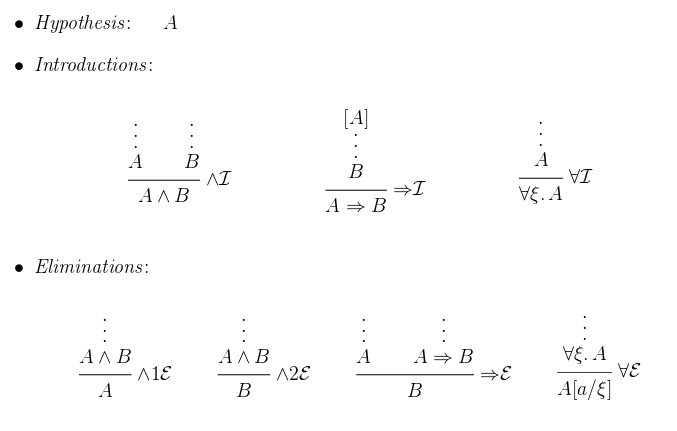
\includegraphics[width=0.9\textwidth]{nd_rules.png}
\caption{Fonte: \cite{girard1989}}
\end{figure}

\end{frame}

%------------------------------------------------

\begin{frame}{Exemplo}

Proposição: $ (B \land A) \Rightarrow (A \land B)$

Prova:

\begin{prooftree}
\AxiomC{[$B \land A$]}
\RightLabel{$\land 2 \mathcal{E}$}
\UnaryInfC{$A$}
\AxiomC{[$B \land A $]}
\RightLabel{$\land 1 \mathcal{E}$}
\UnaryInfC{$B$}
\RightLabel{$\land \mathcal{I}$}
\BinaryInfC{$A \land B$}
\RightLabel{$\Rightarrow \mathcal{I}$}
\UnaryInfC{$(B \land A) \Rightarrow (A \land B)$}
\end{prooftree}


\end{frame}

%------------------------------------------------

\subsection{Simplificanto Provas}

\begin{frame}{Simplificando Provas}

\begin{columns}
\column{0.5\linewidth}
\centering

\begin{prooftree}
\AxiomC{[$A$]}
\Deduce$\fCenter B$
\RightLabel{$\Rightarrow \mathcal{I}$}
\UnaryInfC{$A \Rightarrow B$}
\AxiomC{}
\Deduce$\fCenter A$
\RightLabel{$\Rightarrow \mathcal{E}$}
\BinaryInfC{$B$}
\end{prooftree}

\column{0.5\linewidth}
\begin{prooftree}
\AxiomC{}
\Deduce$ \fCenter $
\noLine
\UnaryInfC{A}
\Deduce$ \fCenter $
\noLine
\UnaryInfC{B}
\end{prooftree}

\end{columns}

\end{frame}

%------------------------------------------------

\begin{frame}{Simplificando Provas}

\begin{columns}
\column{0.5\linewidth}
\centering

\begin{prooftree}
\AxiomC{}
\Deduce$ \fCenter $
\noLine
\UnaryInfC{$A$}
\AxiomC{}
\Deduce$ \fCenter $
\noLine
\UnaryInfC{$B$}
\RightLabel{$\land \mathcal{I}$}
\BinaryInfC{$A \land B$}
\RightLabel{$\land 1 \mathcal{E}$}
\UnaryInfC{$A$}
\end{prooftree}

\column{0.5\linewidth}
\begin{prooftree}
\AxiomC{}
\Deduce$ \fCenter $
\noLine
\UnaryInfC{A}
\end{prooftree}

\end{columns}

\end{frame}

%------------------------------------------------

\begin{frame}{Simplificando Provas}

\begin{prooftree}
\AxiomC{[$B \land A$]}
\RightLabel{$\land 2 \mathcal{E}$}
\UnaryInfC{$A$}
\AxiomC{[$B \land A $]}
\RightLabel{$\land 1 \mathcal{E}$}
\UnaryInfC{$B$}
\RightLabel{$\land \mathcal{I}$}
\BinaryInfC{$A \land B$}
\RightLabel{$\Rightarrow \mathcal{I}$}
\UnaryInfC{$(B \land A) \Rightarrow (A \land B)$}
\AxiomC{[$B$]}
\AxiomC{[$A$]}
\RightLabel{$\land \mathcal{I}$}
\BinaryInfC{$B \land A$}
\RightLabel{$\Rightarrow \mathcal{E}$}
\BinaryInfC{$A \land B $}

\end{prooftree}

\end{frame}

%------------------------------------------------

\begin{frame}{Simplificando Provas}

\begin{prooftree}
\AxiomC{\textcolor{red}{[$B \land A$]}}
\RightLabel{$\land 2 \mathcal{E}$}
\UnaryInfC{$A$}
\AxiomC{\textcolor{red}{[$B \land A $]}}
\RightLabel{$\land 1 \mathcal{E}$}
\UnaryInfC{$B$}
\RightLabel{$\land \mathcal{I}$}
\BinaryInfC{$A \land B$}
\RightLabel{\textcolor{blue}{$\Rightarrow \mathcal{I}$}}
\UnaryInfC{\textcolor{red}{$(B \land A) \Rightarrow (A \land B)$}}
\AxiomC{[$B$]}
\AxiomC{[$A$]}
\RightLabel{$\land \mathcal{I}$}
\BinaryInfC{\textcolor{red}{$B \land A$}}
\RightLabel{\textcolor{blue}{$\Rightarrow \mathcal{E}$}}
\BinaryInfC{$A \land B $}

\end{prooftree}

\end{frame}

%------------------------------------------------

\begin{frame}{Simplificando Provas}

\begin{columns}
\column{0.5\linewidth}
\centering

\begin{prooftree}
\AxiomC{\textcolor{red}{[$B \land A$]}}
\RightLabel{$\land 2 \mathcal{E}$}
\UnaryInfC{$A$}
\AxiomC{\textcolor{red}{[$B \land A $]}}
\RightLabel{$\land 1 \mathcal{E}$}
\UnaryInfC{$B$}
\RightLabel{$\land \mathcal{I}$}
\BinaryInfC{$A \land B$}
\RightLabel{\textcolor{blue}{$\Rightarrow \mathcal{I}$}}
\UnaryInfC{\textcolor{red}{$(B \land A) \Rightarrow (A \land B)$}}
\AxiomC{[$B$]}
\AxiomC{[$A$]}
\RightLabel{$\land \mathcal{I}$}
\BinaryInfC{\textcolor{red}{$B \land A$}}
\RightLabel{\textcolor{blue}{$\Rightarrow \mathcal{E}$}}
\BinaryInfC{$A \land B $}

\end{prooftree}

\column{0.5\linewidth}

\begin{prooftree}
\AxiomC{[$B$]}
\AxiomC{[$A$]}
\BinaryInfC{$B \land A$}
\Deduce$ \fCenter $
\noLine
\UnaryInfC{$A \land B$}
\end{prooftree}

\end{columns}

\end{frame}

%------------------------------------------------

\begin{frame}{Simplificando Provas}

\begin{columns}
\column{0.5\linewidth}
\centering

\begin{prooftree}
\AxiomC{[$B$]}
\AxiomC{[$A$]}
\RightLabel{\textcolor{red}{$\land \mathcal{I}$}}
\BinaryInfC{$B \land A$}
\RightLabel{\textcolor{red}{$\land 2 \mathcal{E}$}}
\UnaryInfC{\textcolor{red}{$A$}}
\AxiomC{[$B$]}
\AxiomC{[$A$]}
\RightLabel{\textcolor{blue}{$\land \mathcal{I}$}}
\BinaryInfC{$B \land A$}
\RightLabel{\textcolor{blue}{$\land 1 \mathcal{E}$}}
\UnaryInfC{\textcolor{blue}{$B$}}
\BinaryInfC{$A \land B$}

\end{prooftree}

\column{0.5\linewidth}

\begin{prooftree}
\AxiomC{}
\end{prooftree}

\end{columns}

\end{frame}

%------------------------------------------------

\begin{frame}{Simplificando Provas}

\begin{columns}
\column{0.5\linewidth}
\centering

\begin{prooftree}
\AxiomC{[$B$]}
\AxiomC{[$A$]}
\RightLabel{$\land \mathcal{I}$}
\BinaryInfC{$B \land A$}
\RightLabel{$\land 2 \mathcal{E}$}
\UnaryInfC{$A$}
\AxiomC{[$B$]}
\AxiomC{[$A$]}
\RightLabel{$\land \mathcal{I}$}
\BinaryInfC{$B \land A$}
\RightLabel{$\land 1 \mathcal{E}$}
\UnaryInfC{$B$}
\BinaryInfC{$A \land B$}

\end{prooftree}

\column{0.5\linewidth}

\begin{prooftree}
\AxiomC{$[A]$}
\AxiomC{$[B]$}
\RightLabel{$\land \mathcal{I}$}
\BinaryInfC{$A \land B$}
\end{prooftree}

\end{columns}

\end{frame}

%------------------------------------------------
\section{Sequent Calculus}
%------------------------------------------------

\begin{frame}{Sequent Calculus}

Baseado (roubado!) no tutorial interativo de \cite{yanglogitext2012}.

\end{frame}

%------------------------------------------------
\section{Lambda-Cálculo}
%------------------------------------------------

\begin{frame}{$\lambda$-Cálculo}

\begin{block}{}

\begin{align*}
s &::=  x \mid (\lambda x.s) \mid (s ~ s)
\end{align*}
onde $x$ é uma variável atômica.

\end{block}

\end{frame}

%------------------------------------------------

\begin{frame}{$\lambda$-Cálculo como Lógica}

\begin{block}{Combinador Y}
\vskip2mm
\begin{equation}
Y = \lambda f.(\lambda x.(f (x x)) ~\lambda x.(x x))
\end{equation}
\vskip2mm

Descoberto por Haskell Curry.

\end{block}

\end{frame}

%------------------------------------------------

\begin{frame}{Paradoxos = Loops Infinitos}

\begin{exampleblock}{}
\justify
  {\large ``Whereas self-application in Russell’s logic leads to paradox, self-application in Church’s untyped $\lambda$-calculus leads to non-terminating computations.''}
  \vskip5mm
  \hspace*\fill{\small--- Propositions as Types, Wadler}
\end{exampleblock}

\end{frame}

%------------------------------------------------
\section{Lambda-Cálculo Simplesmente Tipado}
%------------------------------------------------

\begin{frame}{$\lambda$-Cálculo Simplesmente Tipado}

\begin{columns}
\column{0.38\linewidth}
\centering
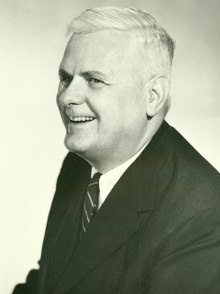
\includegraphics[width=4cm]{church.jpg}
\column{0.58\linewidth}
\textbf{Alonzo Church, 1903 - 1995.}\\
\justifying
‘There may, indeed, be other applications of the system than its use as a logic.’
\end{columns} 

\end{frame}

%------------------------------------------------

\begin{frame}{$\lambda$-Cálculo Simplesmente Tipado}

\begin{columns}
\column{0.5\linewidth}
\centering

\begin{prooftree}
\AxiomC{[$x : A$]}
\Deduce$N : \fCenter ~B$
\RightLabel{$\Rightarrow \mathcal{I}$}
\UnaryInfC{$\lambda x.N : A \Rightarrow B$}
\end{prooftree}

\column{0.5\linewidth}

\begin{prooftree}
\AxiomC{$L : A \Rightarrow B$}
\AxiomC{$M : A$}
\RightLabel{$\Rightarrow \mathcal{E}$}
\BinaryInfC{$N : B$}
\end{prooftree}

\end{columns}

\end{frame}

%------------------------------------------------

\begin{frame}{$\lambda$-Cálculo Simplesmente Tipado}


\begin{columns}
\column{0.3\linewidth}
\centering

\begin{prooftree}
\AxiomC{$M : A$}
\AxiomC{$N : B$}
\RightLabel{$\land \mathcal{I}$}
\BinaryInfC{$(M,N) : A \land B$}
\end{prooftree}

\column{0.3\linewidth}

\begin{prooftree}
\AxiomC{$L : A \land B$}
\RightLabel{$\land 1 \mathcal{E}$}
\UnaryInfC{$\texttt{fst } L : A $}
\end{prooftree}

\column{0.3\linewidth}

\begin{prooftree}
\AxiomC{$L : A \land B$}
\RightLabel{$\land 2 \mathcal{E}$}
\UnaryInfC{$\texttt{snd } L : B $}
\end{prooftree}

\end{columns}

\end{frame}

%------------------------------------------------

\begin{frame}{$\lambda$-Cálculo Simplesmente Tipado}


\begin{columns}
\column{0.5\linewidth}
\centering

\begin{prooftree}
\AxiomC{[$x : \textcolor{red}{A}$]}
\Deduce$N : \fCenter ~\textcolor{red}{B}$
\RightLabel{$\Rightarrow \mathcal{I}$}
\UnaryInfC{$\lambda x.N : \textcolor{red}{A \Rightarrow B}$}
\end{prooftree}

\column{0.5\linewidth}

\begin{prooftree}
\AxiomC{$L : \textcolor{red}{A \Rightarrow B}$}
\AxiomC{$M : \textcolor{red}{A}$}
\RightLabel{$\Rightarrow \mathcal{E}$}
\BinaryInfC{$N : \textcolor{red}{B}$}
\end{prooftree}

\end{columns}


\end{frame}

%------------------------------------------------

\begin{frame}{$\lambda$-Cálculo Simplesmente Tipado}


\begin{columns}
\column{0.3\linewidth}
\centering

\begin{prooftree}
\AxiomC{$M : \textcolor{red}{A}$}
\AxiomC{$N : \textcolor{red}{B}$}
\RightLabel{$\land \mathcal{I}$}
\BinaryInfC{$(M,N) : \textcolor{red}{A \land B}$}
\end{prooftree}

\column{0.3\linewidth}

\begin{prooftree}
\AxiomC{$L : \textcolor{red}{A \land B}$}
\RightLabel{$\land 1 \mathcal{E}$}
\UnaryInfC{$\texttt{fst } L : \textcolor{red}{A} $}
\end{prooftree}

\column{0.3\linewidth}

\begin{prooftree}
\AxiomC{$L : \textcolor{red}{A \land B}$}
\RightLabel{$\land 2 \mathcal{E}$}
\UnaryInfC{$\texttt{snd } L : \textcolor{red}{B}$}
\end{prooftree}

\end{columns}

\end{frame}

%------------------------------------------------

\begin{frame}{Programa}

\begin{prooftree}
\AxiomC{$z : B \land A$}
\RightLabel{$\land 2 \mathcal{E}$}
\UnaryInfC{$\texttt{snd } z : A$}
\AxiomC{$z : B \land A$}
\RightLabel{$\land 1 \mathcal{E}$}
\UnaryInfC{$\texttt{fst } z : B$}
\RightLabel{$\land \mathcal{I}$}
\BinaryInfC{$(\texttt{snd } z, \texttt{fst z}) : (A \land B)$}
\RightLabel{$\Rightarrow \mathcal{I}$}
\UnaryInfC{$\lambda z.(\texttt{snd z}, \texttt{fst z}) : (B \land A) \Rightarrow (A \land B) $}
\end{prooftree}

\end{frame}

%------------------------------------------------

\begin{frame}{Valorando programas}

\begin{columns}
\column{0.4\linewidth}
\centering

\begin{prooftree}
\AxiomC{[$x : A$]}
\Deduce$N : \fCenter ~B$
\RightLabel{$\Rightarrow \mathcal{I}$}
\UnaryInfC{$\lambda x.N : A \Rightarrow B$}
\AxiomC{}
\Deduce$M : \fCenter ~A$
\RightLabel{$\Rightarrow \mathcal{E}$}
\BinaryInfC{$(\lambda x.N)~ M : B$}
\end{prooftree}

\column{0.4\linewidth}

\begin{prooftree}
\AxiomC{}
\Deduce$ \fCenter $
\noLine
\UnaryInfC{$M : A$}
\Deduce$ \fCenter $
\noLine
\UnaryInfC{$N\{M / x \} : B$}
\end{prooftree}

\end{columns}

\end{frame}

%------------------------------------------------

\begin{frame}{Valorando programas}

\begin{columns}
\column{0.4\linewidth}
\centering

\begin{prooftree}
\AxiomC{}
\Deduce$M : \fCenter ~A $
\AxiomC{}
\Deduce$N : \fCenter ~B $
\RightLabel{$\land \mathcal{I}$}
\BinaryInfC{$(M,N) : A \land B$}
\RightLabel{$\land 1 \mathcal{E}$}
\UnaryInfC{$\texttt{fst } (M,N) : A$}
\end{prooftree}

\column{0.4\linewidth}

\begin{prooftree}
\AxiomC{}
\Deduce$M : \fCenter ~A$
\end{prooftree}

\end{columns}

\end{frame}


%------------------------------------------------

\begin{frame}{A diferença entre os dois Cálculos}
\begin{columns}
\column{0.38\linewidth}
\centering
\begin{figure}
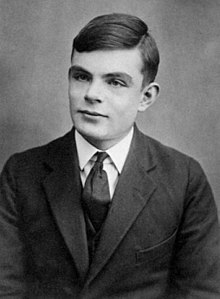
\includegraphics[width=4cm]{turing.jpg}
\caption*{Alan Turing, 1912 - 1954.}
\end{figure}
\column{0.58\linewidth}
\textbf{An early proof of normalization. }\\
\justifying
O $\lambda$-Cálculo não tipado permite a definição de qualquer função efetivamente computável, mas possui um problema da parada insolúvel. Em contrapartida, o $\lambda$-Cálculo sem recursão geral ($\textit{general recursion}$) possui um Problema da Parada trivial, pois todo programa termina, mas não consegue representar todas as funções computáveis.

\end{columns} 
\end{frame}




%------------------------------------------------
\section{O Isomorfismo de Curry-Howard}
%------------------------------------------------

\begin{frame}{Curry-Howard}

\begin{exampleblock}{}
\justifying
  {\large ``Algorithms are the computational content of proofs.''}
  \vskip5mm
  \hspace*\fill{\small--- Robert Harper}
\end{exampleblock}

\begin{exampleblock}{}
\justifying
  {\large ``Curry–Howard is a double-barreled name that ensures the existence of other double-barreled names.''}
  \vskip5mm
  \hspace*\fill{\small--- Philip Wadler}
\end{exampleblock}

\end{frame}

%------------------------------------------------

\begin{frame}{Conjunção}

“$A \land B$ corresponds to Cartesian product $A \times B$,
that is, a record with two fields, also known as a
pair. A proof of the proposition $A \land B$ consists of a
proof of $A$ and a proof of $B$. Similarly, a value of
type $A \times B$ consists of a value of type $A$ and a
value of type $B$.”

\end{frame}

%------------------------------------------------

\begin{frame}{Disjunção}

“$A \lor B$ corresponds to a disjoint sum $A + B$, that
is, a variant with two alternatives. A proof of the
proposition $A \lor B$ consists of either a proof of $A$
or a proof of $B$, including an indication of which
of the two has been proved. Similarly, a value of
type $A + B$ consists of either a value of type $A$ or
a value of type $B$, including an indication of
whether this is a left or right summand.”

\end{frame}

%------------------------------------------------

\begin{frame}{Implicação}

“$A \Rightarrow B$ corresponds to function space $A \rightarrow B$. A proof of the proposition $A \Rightarrow B$ consists of a procedure that given a proof of $A$ yields a proof of $B$. Similarly, a value of type $A \rightarrow B$ consists of a function that when applied to a value of type $A$ returns a value of type $B$.”

\end{frame}

%------------------------------------------------

\begin{frame}{$P \land (Q \lor R) \Rightarrow (P \land Q) \lor (P \land R) $}

\begin{columns}
\column{0.3\linewidth}
\centering

\begin{align*}
A \land B &\longmapsto A \times B
\end{align*}

\begin{prooftree}
\AxiomC{$x : A$}
\AxiomC{$y : B$}
\BinaryInfC{$(x,y) : A \times B$}
\end{prooftree}

\column{0.3\linewidth}

\begin{align*}
A \lor B &\longmapsto A + B
\end{align*}

\begin{prooftree}
\AxiomC{$x : A$}
\UnaryInfC{$\texttt{Left } x : (A + B)$}
\end{prooftree}

\begin{prooftree}
\AxiomC{$y : B$}
\UnaryInfC{$\texttt{Right } y : (A + B)$}
\end{prooftree}

\column{0.3\linewidth}

\begin{align*}
A \Rightarrow B &\longmapsto A \rightarrow B
\end{align*}

Construir uma função $f : A \rightarrow B$.

\end{columns}

\end{frame}

%------------------------------------------------

\begin{frame}{$P \times (Q + R) \rightarrow (P \times Q) + (P \times R) $}

\begin{align*}
f (x, ~\texttt{Left } y) &= \texttt{Left } (x, y)\\
f (x, ~\texttt{Right } z) &= \texttt{Right } (x, z) 
\end{align*}

\end{frame}


%------------------------------------------------

\begin{frame}{Isomorfismos}

\begin{block}{}

\begin{center}
\begin{tabular}{ c c c }
\pause
 Dedução Natural & $\longleftrightarrow$ & $\lambda$-Cálculo Tipado \\ 
 (Gentzen, 1935) &  & (Church, 1940) \\  
                 &  &  \\
\pause 
 Type Schemes & $\longleftrightarrow$ & Sistema de Tipos da ML \\ 
 (Hindley, 1969) &  & (Milner, 1975) \\  
                 &  &  \\
\pause
 System F & $\longleftrightarrow$ & $\lambda$-Cálculo Polimórfico \\ 
 (Girard, 1972) &  & (Reynolds, 1974) \\  
                &  &  \\
\pause
 Lógica Modal & $\longleftrightarrow$ & Mônadas \\ 
 (Lewis, 1910) &  & (Kleisi, 1965), (Moggi, 1987) \\  
               &  &    \\
\pause
 Classical-Intuitionistic Embedding & $\longleftrightarrow$ & Continuation Passing Style \\ 
 (Gödel, 1933) &  & (Reynolds, 1972) \\  
               &  &   
\end{tabular}
\end{center}

\end{block}

\end{frame}

%------------------------------------------------

\begin{frame}{A vingança de Reynolds!}

\begin{block}{}

\begin{center}
\begin{tabular}{ c c c }
 Lógica Linear & $\longleftrightarrow$ & Syntatic Control of Interference \\ 
 (Girard, 1987) &  & (Reynolds, 1978) \\  
                 &  &  \\
 Lógica Linear & $\longleftrightarrow$ & Session Types \\ 
 (Girard, 1987) &  & (Honda, 1993) \\  
                 &  &      
\end{tabular}
\end{center}

\end{block}

\end{frame}

%------------------------------------------------

\begin{frame}{Coq}

Learning resources:

\begin{itemize}
\item \href{https://softwarefoundations.cis.upenn.edu/}{Software Foundations}
\item \href{https://math-comp.github.io/mcb/}{Mathematical Components}
\end{itemize}

\end{frame}

%------------------------------------------------

\section{Conclusão}

\begin{frame}{Conclusão}

\begin{block}{}

\[
\begin{array}{rcccl}
\textsf{PROGRAMS} & \Longleftrightarrow & \textsf{LOGIC} & \Longleftrightarrow & \textsf{CATEGORIES}\\
\textsf{type} & \Longleftrightarrow & \textsf{formula} & \Longleftrightarrow & \textsf{object}\\
\textsf{function} & \Longleftrightarrow & \textsf{implication} & \Longleftrightarrow & \textsf{arrow}\\
\textsf{tuple} & \Longleftrightarrow & \textsf{conjunction} & \Longleftrightarrow & \textsf{product}\\
\end{array}
\]

\end{block}

\end{frame}



%------------------------------------------------
% Bibliography
%------------------------------------------------

\begin{frame}[allowframebreaks]
\frametitle{Referências}
\footnotesize{
\begin{thebibliography}{99}
\bibitem[Wadler, 2015]{wadlertypes15} Philip Wadler (2015)
\newblock Propositions as types
\newblock \emph{Communications of the ACM} 58(12), 75 -- 84.

\bibitem[Church, 1936]{church1936unsolvable} Alonzo Church (1936)
\newblock An unsolvable problem of elementary number theory
\newblock \emph{American journal of mathematics} 58(2), 345 -- 363.

\bibitem[Kleene, 1936]{kleene1936general} Stephen Cole Kleene (1936)
\newblock General recursive functions of natural numbers
\newblock \emph{Mathematische annalen} 112(1), 727 -- 742.

\bibitem[Turing, 1936]{turing1937computable} Alan M. Turing (1936)
\newblock On computable numbers, with an application to the Entscheidungsproblem
\newblock \emph{Proceedings of the London mathematical society} 2(1), 230 -- 265.

\bibitem[Girard, 1989]{girard1989} Girard, Jean-Yves and Taylor, Paul and Lafont, Yves (1989)
\newblock Proofs and Types
\newblock \emph{Cambridge University Press Cambridge} 7.

\bibitem[Yang, 2012]{yanglogitext2012} Edward Z. Yang, (2012)
\newblock Logitext Tutorial
\newblock \emph{\href{http://logitext.mit.edu/tutorial}{http://logitext.mit.edu/tutorial}}.

\end{thebibliography}
}
\end{frame}

%----------------------------------------------------------------------------------------

\end{document}